\documentclass[11pt]{article}

\usepackage[margin=1.0in]{geometry}

\usepackage{amsmath}
\numberwithin{equation}{section}
\numberwithin{figure}{section}
\numberwithin{table}{section}

\usepackage{sectsty}
\sectionfont{\centering \normalsize}
\subsectionfont{\centering \small}
\subsubsectionfont{\centering \small \textit}
\usepackage{caption}
\captionsetup[figure]{labelsep=quad, labelfont=bf, width=\linewidth}

\usepackage{mathtools}
\usepackage[inline]{enumitem}
\usepackage{booktabs}
\usepackage{graphicx}
\usepackage{amssymb}
\usepackage{amsthm}
\newtheorem{definition}{Definition}
\numberwithin{definition}{section}

\usepackage[sort&compress]{natbib}
\bibliographystyle{apsrev}
\renewcommand{\bibsep}{0pt}
\newcommand{\eprint}[1]{\href{http://arxiv.org/abs/#1}{#1}}

\renewcommand\thesection{\Roman{section}}
\renewcommand\thesubsection{\Alph{subsection}}
\renewcommand\thefigure{\arabic{section}.\arabic{figure}}
\renewcommand\theequation{\arabic{section}.\arabic{equation}}
\renewcommand\thedefinition{\arabic{section}.\arabic{definition}}

\renewcommand\labelitemi{\raisebox{0.25ex}{\tiny$\bullet$}}

\usepackage{color}
\usepackage[colorlinks]{hyperref}
\hypersetup{colorlinks=true, urlcolor=cyan, citecolor=cyan, runcolor=black, menucolor=black, filecolor=black, anchorcolor=black, linkcolor=black}

\usepackage[protrusion=true]{microtype}
\usepackage{breqn}
\usepackage{slashed}

\setcounter{tocdepth}{2}

\renewcommand\vec{\mathbf}
\newcommand{\normord}[1]{\raisebox{0.5pt}{:}\,#1\,\raisebox{0.5pt}{:}}
\newcommand{\dagg}{^{\dagger}}
\newcommand{\pr}{^{\prime}}
\newcommand{\nhat}{\hat{\bm{n}}}
\newcommand{\hamilt}{\mathcal{H}}
\newcommand{\mA}{\mathcal{A}}
\newcommand{\mW}{\mathcal{W}}
\newcommand{\mN}{\mathcal{N}}
\newcommand{\mD}{\mathcal{D}}
\newcommand{\mS}{\mathcal{S}}
\newcommand{\mL}{\mathcal{L}}
\newcommand{\mC}{\mathcal{C}}
\newcommand{\mO}{\mathcal{O}}
\newcommand{\mM}{\mathcal{M}}
\newcommand{\mT}{\mathcal{T}}
\newcommand{\mZ}{\mathcal{Z}}
\newcommand{\mR}{\mathcal{R}}
\newcommand{\II}{\mathbb{I}}
\newcommand{\RR}{\mathbb{R}}
\newcommand{\ZZ}{\mathbb{Z}}
\newcommand{\CC}{\mathbb{C}}
\newcommand{\FF}{\mathbb{F}}
\newcommand{\lie}[1]{\mathcal{L}\left(#1\right)}
\newcommand{\set}[1]{\left\{#1\right\}}
\newcommand{\SO}[1]{\textrm{SO}\left(#1\right)}
\newcommand{\SU}[1]{\textrm{SU}\left(#1\right)}
\newcommand{\Orth}[1]{\textrm{O}\left(#1\right)}
\newcommand{\Uni}[1]{\textrm{U}\left(#1\right)}
\newcommand{\paraskip}{\vspace{10pt}}
\newcommand{\del}{\partial}
\newcommand{\TeG}{\mathcal{T}_e(\mathscr{G})}
\newcommand{\TpM}{\mathcal{T}_p(\mathcal{M})}
\newcommand{\TpMs}{\mathcal{T}^{\star}_p(\mathcal{M})}
\newcommand{\etamn}[1]{\eta#1{\mu \nu}}
\newcommand{\upd}[1]{\text{d}#1 \,}
\newcommand{\ud}{\text{d}}
\newcommand{\group}{\mathscr{G}}
\newcommand{\alge}{\mathfrak{g}}
\newcommand{\twobytwo}[4]{\begin{pmatrix}#1&#2 \\ #3&#4 \end{pmatrix}}
\newcommand{\thrbythr}[3]{\begin{pmatrix}#1 \\ #2 \\ #3\end{pmatrix}}
\newcount\colveccount
\newcommand*\colvec[1]{
        \global\colveccount#1
        \begin{pmatrix}
        \colvecnext
}
\def\colvecnext#1{
        #1
        \global\advance\colveccount-1
        \ifnum\colveccount>0
                \\
                \expandafter\colvecnext
        \else
                \end{pmatrix}
        \fi
}
\newcommand{\Abs}[1]{\left| #1 \right|}
\newcommand{\tr}{\text{Tr}}
\usepackage{breqn}

\title{\textbf{CMBGraph: A new data representation of the Cosmic Microwave Background}}
\author{J.B.G. Alvey \\ \textit{\footnotesize Theoretical Particle Physics and Cosmology, King's College London}}
\date{}

\begin{document}
\maketitle
\abstract{The most precise measurement of the Cosmic Microwave Background (CMB) comes from space-bound satellites such as WMAP \citep{Hinshaw:2012aka} and the Planck satellite \citep{Aghanim:2018eyx}. This consists of temperature and polarisation data measured against a uniform temperature background of approximately 2.73 $\mathrm{K}$. An important quantity that can be measured from the maps is the angular power spectra. These play a high-precision role in constraining theories of inflation and cosmological evolution. This letter considers a new representation of this data in terms of a planar graph which aims to encode the angular correlation function in a more complete way compared to the power spectrum. We denote this type of structure a \textit{planar correlation graph}. More recently \citep{DBLP:journals/corr/abs-1806-01261}, there has been interest in a new network architecture for Deep Learning known as a Graph Network. Input to this network is in the form of a planar graph. Whilst we are not advocating the use of a Graph network at this stage for Cosmology, the abstraction of the CMB data to a higher dimensional graph is a natural step forwards. The weighting of the edges of the graph using the power spectrum is then a physically motivated choice for an element of the architecture that is user-defined.}
\vspace*{20pt}
\begin{center}
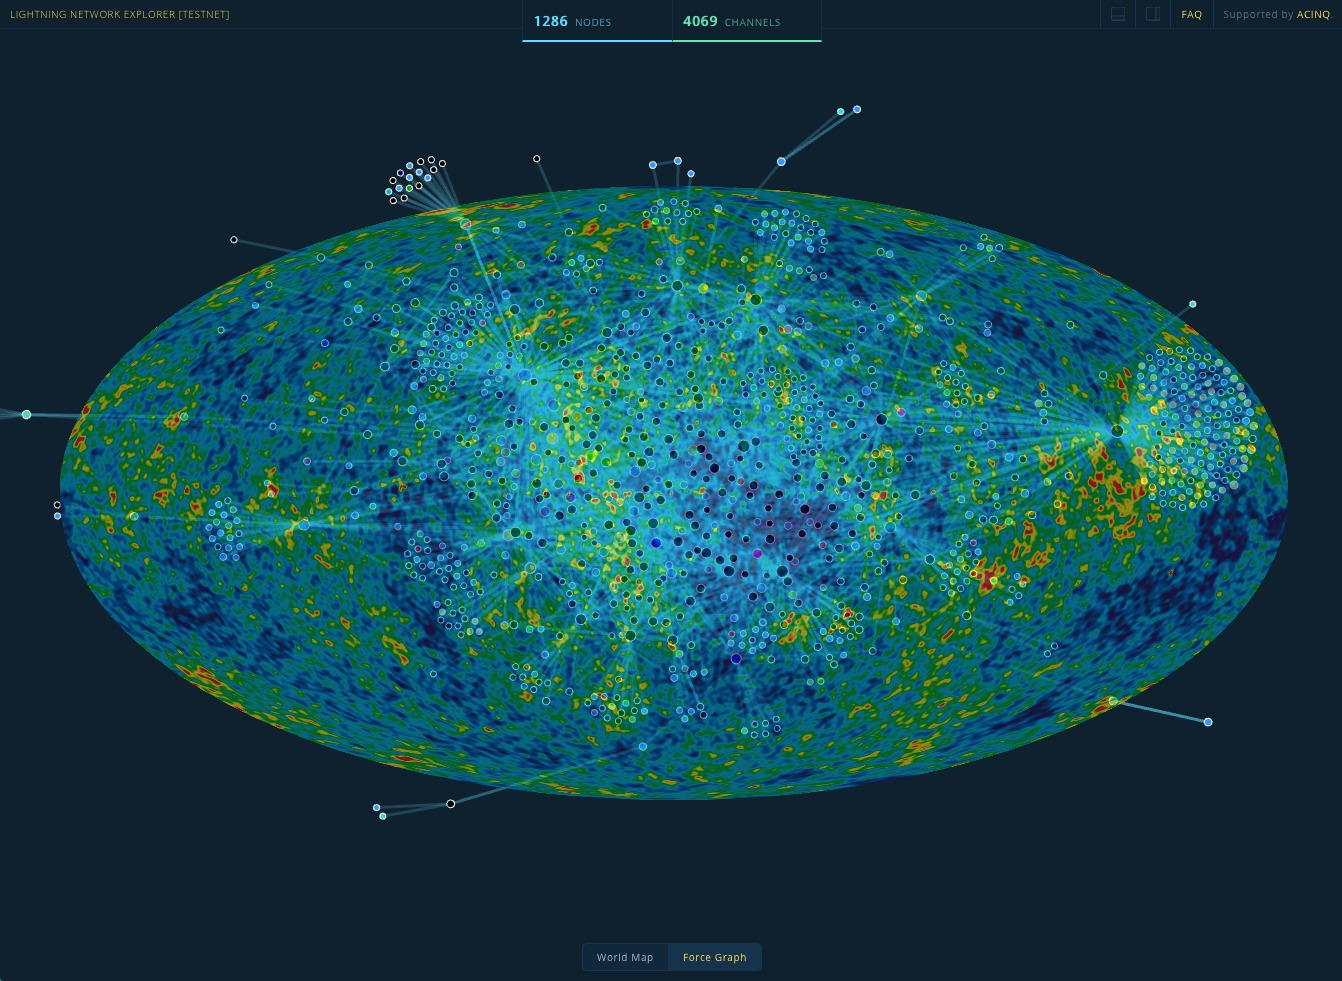
\includegraphics[width=0.7\linewidth]{overlay.jpg}
\end{center}
\renewcommand{\thefootnote}{\arabic{footnote}}
\newpage



\section{The Ising Model in 1D}



The Ising model is the prototypical example of a statistical system whose correlations and fluctuations lead to non-trivial phenomenology beyond that suggested by the mean field solution. We will use this example as a warm up to the case of the full CMB. We will illustrate how to construct the planar graphs based on the correlation function which is simple to state in this setup. In one dimension, the Ising model is a set of spins, $\{\sigma_i\}$ on a line of sites labelled $i = 1, 2, \cdots N$. Note that we are not necessarily assuming periodic boundary conditions in this case. The Hamiltonian for the system is then given by,
\begin{equation}
\mathcal{H} = -J \sum_{i = 1}^{N}{\sigma_i \sigma_{i + 1}} - H \sum_{i = 1}^{N}{\sigma_i},
\end{equation}
from which we can compute the canonical partition function,
\begin{equation}
Z_N = \sum_{\{\sigma_i\}}{\exp\left(\beta J \sum_{i = 1}^{N}{\sigma_i \sigma_{i + 1}} + \beta H\sum_{i = 1}^{N}{\sigma_i}\right)}.
\end{equation}
Now, for a given system, $J$ and $H$ are typically fixed and characterise the strength of the interactions and the energy of the spin state due to an external field respectively. Furthermore, $\beta = 1/T$ can vary with the temperature.\footnote{$k_B = 1$ here.} The key physics of the Ising model in our context is the fact that correlations/fluctuations between the spin sites destroy the long range order that would be characteristic of a phase transition at low temperature. An argument by Landau demonstrated that indeed there is no phase transition in the 1D Ising model despite the mean field solution suggesting otherwise. When $H = 0$, it is possible to calculate the correlation function (which is discrete in this case), and one finds,
\begin{equation}
\langle \sigma_i \sigma_j \rangle = \frac{1}{Z_N}\sum_{\{\sigma_i\}}{\sigma_i \sigma_j \exp(-\beta \mathcal{H})} = \exp\left(\Abs{i - j}\log(\tanh\beta J)\right).
\end{equation}
The behaviour of the correlation as a function of the site separation is shown in Figure \ref{fig:isingcorrelation} for $N = 20$ sites. This is now in a suitable form to illustrate the concept of a planar correlation graph. In the case of the Ising model it is constructed as follows,
\begin{figure}[h]
\begin{center}
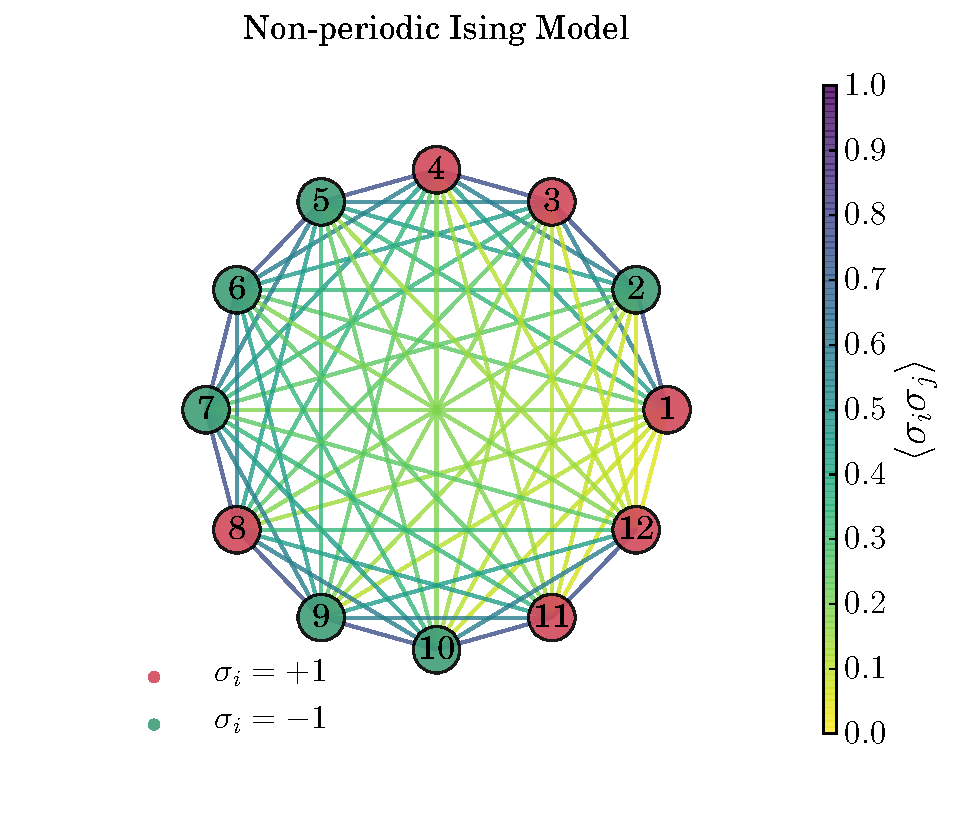
\includegraphics[width=0.49\linewidth]{figures/non_periodic.pdf} \hfill
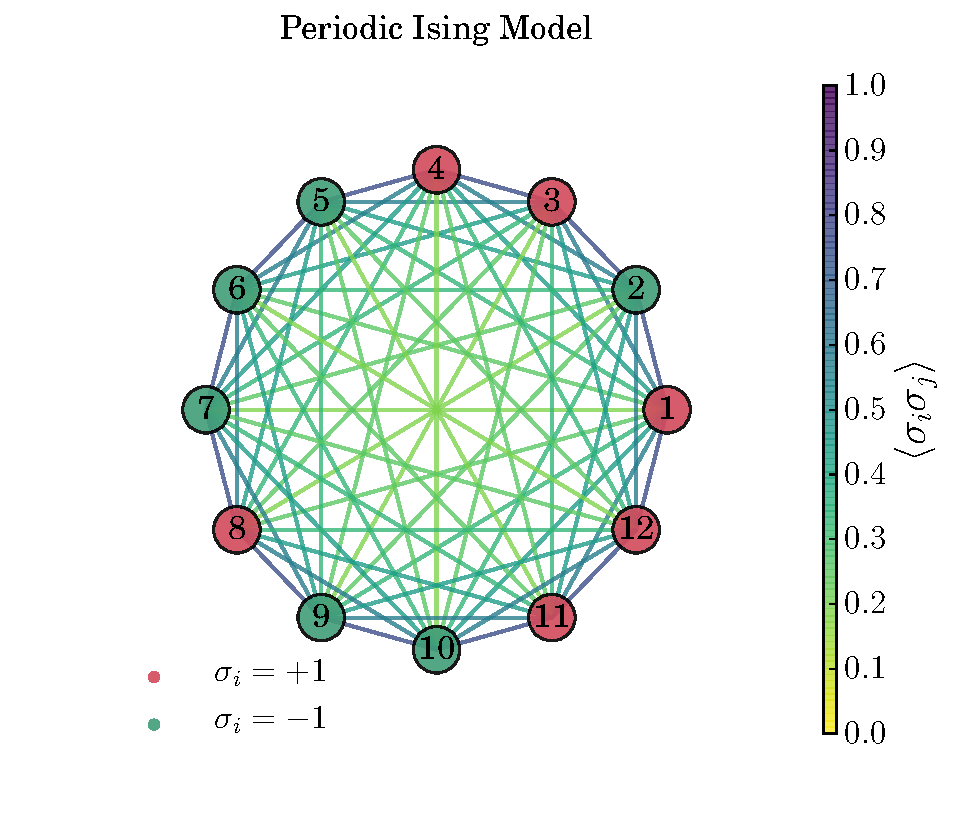
\includegraphics[width=0.49\linewidth]{figures/periodic.pdf}
\caption{The planar correlation graphs in the case of the Ising model for $N = 12$ sites, with $\beta J = 1$. This is shown for non-periodic (Left) and periodic (Right) boundary conditions}\label{fig:isinggraphs}
\end{center}
\end{figure}
% \begin{figure}[t]
% \begin{center}
% 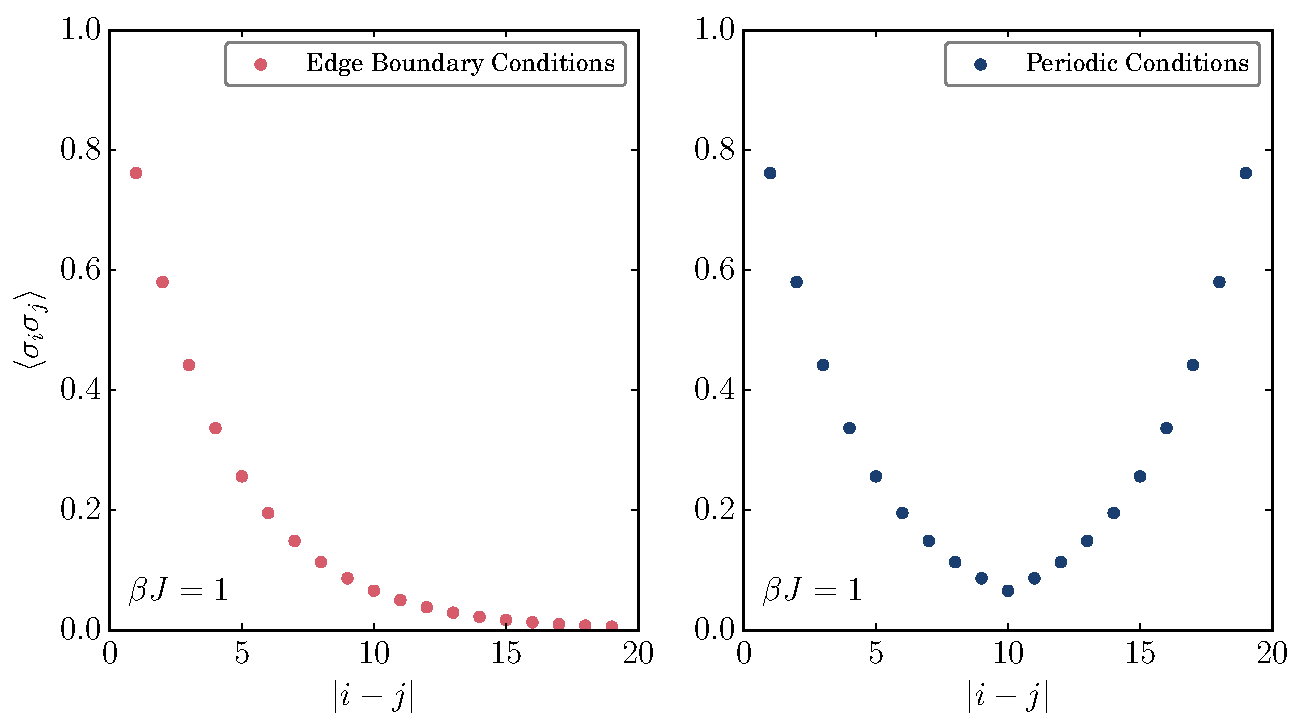
\includegraphics[width=0.8\linewidth]{figures/ising_correlation.pdf}
% \caption{Plots of the correlation function, $\langle \sigma_i \sigma_j \rangle$ in the 1D Ising model for non-periodic (Left) and periodic (Right) boundary conditions.}\label{fig:isingcorrelation}
% \end{center}
% \end{figure}
\begin{enumerate}
        \item To each lattice site $i = 1, 2, \cdots, N$, associate a vertex $v_i$ on the graph, $G$.
        \item At each vertex $v_i$, store the information $(i, \sigma_i)$ in a suitable data structure.
        \item Between vertices $v_i$ and $v_j$, draw an edge $e_{ij}$ weighted according to the correlation function $\langle \sigma_i \sigma_j \rangle$ as computed above.
\end{enumerate}
This procedure will lead to a planar graph $G = \{v_i, e_{ij}\}$ along with a set of weights $\{w_{ij} = \langle \sigma_i \sigma_j \rangle \}$, as well as a map $\mathfrak{D}: V \rightarrow \mathcal{M}$. Here $\mathfrak{D}$ should be viewed as a function from the set of vertices $V$ to a suitabel data manifold, $\mathcal{M}$. In the case of the Ising model for example,
\begin{equation}
\mathfrak{D}: V \rightarrow \mathbb{Z} \times \{-1, 1\}, \,\, \mathfrak{D}(v) \mapsto (i, \sigma_i).
\end{equation}
For the CMB that we will consider later, this map will instead be of the form, $\mathfrak{D}: V \rightarrow S_2 \times \mathbb{R}$, $\mathfrak{D}(v) \rightarrow \left(\hat{\mathbf{n}}, \delta T(\hat{\mathbf{n}})/T_{\textrm{\tiny CMB}}\right)$. We formalise this with the following definition;
\begin{definition}
A \textit{planar correlation graph} is a planar graph $G = \{V, E\}$, formed of a set of edges $E = \{e_{ij}\}$, and a set of vertices $V = \{v_i\}$ together with;
\begin{enumerate}
\item A set of weights $w_{ij}$ that characterise the correlation between the data at the vertex $v_i$ and that at $v_j$.
\item A map $\mathfrak{D}: V \rightarrow \mathcal{M}$, where $\mathcal{M}$ is a suitable data manifold. This places the role of `storing' the data at each vertex (e.g. CMB temperature/polarisation or the spin in the Ising model).
\end{enumerate} 
\end{definition}

We now apply this idea to the explicit example of the Ising model on $N = 12$ lattice sites for both periodic and non-periodic boundary conditions, with $\beta J = 1$. Labelling the nodes as $i \in \{1, 2, \cdots, N\}$, we randomly sample an initial spin state $\{\sigma_i\}$ and display the information via the colour of the nodes. Furthermore, we assign the weight $w_{ij} = \langle \sigma_i \sigma_j \rangle$between site $i$ and site $j$ and indicate this via the colour of the edge on the graph. The results are shown in Figure \ref{fig:isinggraphs}. We see that the graphs encode the different correlation graphs illustrate the difference between the two sets of boundary conditions via the weights.



\section{The Cosmic Microwave Background}



We used the Ising model as an example of how to construct a planar correlation graph. We now wish to extend this idea to the CMB. To understand the correlations of the cosmic microwave background, we should first understand the expansion of a general random field, $f(\hat{\mathbf{n}})$, on a sphere. For such a field, we can expand $f(\hat{\mathbf{n}})$ in terms of spherical harmonics, $Y_{lm}(\hat{\mathbf{n}}) = Y_{lm}(\theta, \phi)$ as follows;
\begin{equation}
f(\hat{\mathbf{n}}) = \sum_{l = 0}^{\infty}{\sum_{m = -l}^{l}{f_{lm} Y_{lm}(\hat{\mathbf{n}})}},
\end{equation}
where the set of $f_{lm}$ are the expansion coefficients. The $Y_{lm}$ are orthogoanl in the sense that,
\begin{equation}
\int{\textrm{d}{\hat{\mathbf{n}}}\,Y_{lm}(\hat{\mathbf{n}})Y^{\star}_{l'm'}(\hat{\mathbf{n}})} = \delta_{ll'}\delta_{mm'},
\end{equation}
so we can extract the expansion coefficients via,
\begin{equation}
f_{lm} = \int{\textrm{d}\hat{\mathbf{n}}\,f(\hat{\mathbf{n}})Y^{\star}_{lm}(\hat{\mathbf{n}})}.
\end{equation}
Now, in the context described in this paper where we wish to abstract the real space, map representation of the CMB, we are interested in spatial correlations. To compute these, we consider
\begin{equation}
\langle f(\hat{\mathbf{n}}) f^{\star}(\hat{\mathbf{n}}')\rangle = \sum_{lm}{\sum_{l'm'}{\langle f_{lm} f^\star_{l'm'}\rangle Y_{lm}(\hat{\mathbf{n}}) Y^{\star}_{l'm'}(\hat{\mathbf{n}}')}}.
\end{equation}
Rotational invariance of the CMB (in our case) implies that $\langle f_{lm} f^\star_{l'm'}\rangle$ must be of the form
\begin{equation}
\langle f_{lm} f^\star_{l'm'}\rangle \equiv C_l \delta_{ll'}\delta_{mm'}.
\end{equation}
So, we can compute the two point correlation function as,
\begin{align*}
\langle f(\hat{\mathbf{n}}) f^{\star}(\hat{\mathbf{n}}')\rangle &= \sum_{lm}{\sum_{l'm'}{\langle f_{lm} f^\star_{l'm'}\rangle Y_{lm}(\hat{\mathbf{n}}) Y^{\star}_{l'm'}(\hat{\mathbf{n}}')}} \\
&= \sum_{l}{C_l\sum_{m}{Y_{lm}(\hat{\mathbf{n}})Y^\star_{lm}(\hat{\mathbf{n}}')}} \\
&= \sum_{l}{\frac{l(l + 1)}{4\pi}C_l P_l(\hat{\mathbf{n}}\cdot\hat{\mathbf{n}}')},
\end{align*}
where we have made use of a standard identity relating the Legendre polynomials, $P_l(\hat{\mathbf{n}}\cdot\hat{\mathbf{n}}') = P_l(\cos\theta)$ and the spherical harmonics, $Y_{lm}(\hat{\mathbf{n}})$. We will now work with the CMB data and consider the field $f(\hat{\mathbf{n}}) = \delta T(\hat{\mathbf{n}})/T_{\textrm{\tiny CMB}}$. The Planck analysis \citep{Aghanim:2018eyx} provides the correlation coefficients $C_l$ in their analysis. From these, we can extract the correlation function, $C(\theta)$, which measures the correlation on some angular scale $\theta$.\footnote{Here, $\theta$ satisfies $\hat{\mathbf{n}}\cdot\hat{\mathbf{n}}' = \cos\theta$.}. This is given by,
\begin{equation}
\left< \frac{\delta T(\hat{\mathbf{n}})}{T_{\textrm{\tiny CMB}}} \frac{\delta T(\hat{\mathbf{n}}')}{T_{\textrm{\tiny CMB}}}\right> = C(\theta) = \sum_{l}{\frac{2l + 1}{4\pi}C_l P_l(\cos\theta)}.
\end{equation}
Plots of both $\mathcal{D}_l := l(l + 1)C_l/2\pi$ as well as $C(\theta)$ are shown in Figure \ref{fig:cmbspectrum}, illustrating the characteristic shapes. We will be mainly interested in $C(\theta)$ as a proxy by which to weight our planar graph.
\begin{figure}[t]
\begin{center}
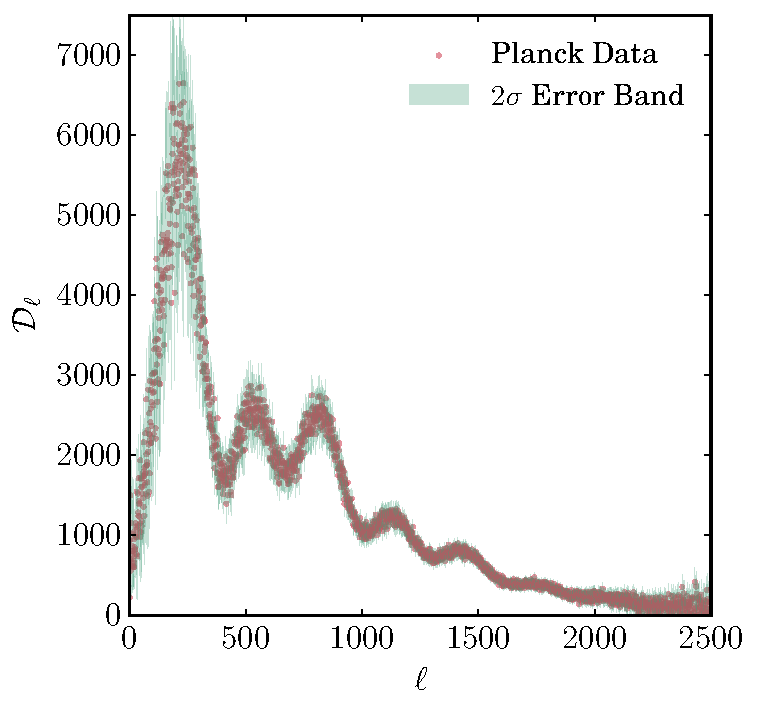
\includegraphics[width=0.49\linewidth]{figures/TTspectrum.pdf} \hfill
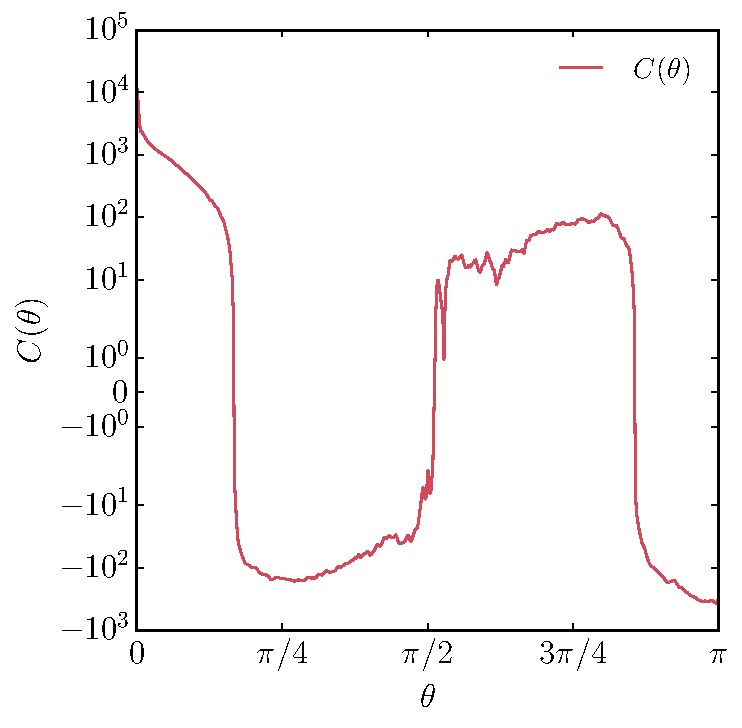
\includegraphics[width=0.49\linewidth]{figures/correlation.pdf}
\caption{Plots of the correlation coefficients, $\mathcal{D}_l$ (Left) and the correlation function, $C(\theta)$ (Right).}\label{fig:cmbspectrum}
\end{center}
\end{figure}

\begin{figure}[t]
\begin{center}
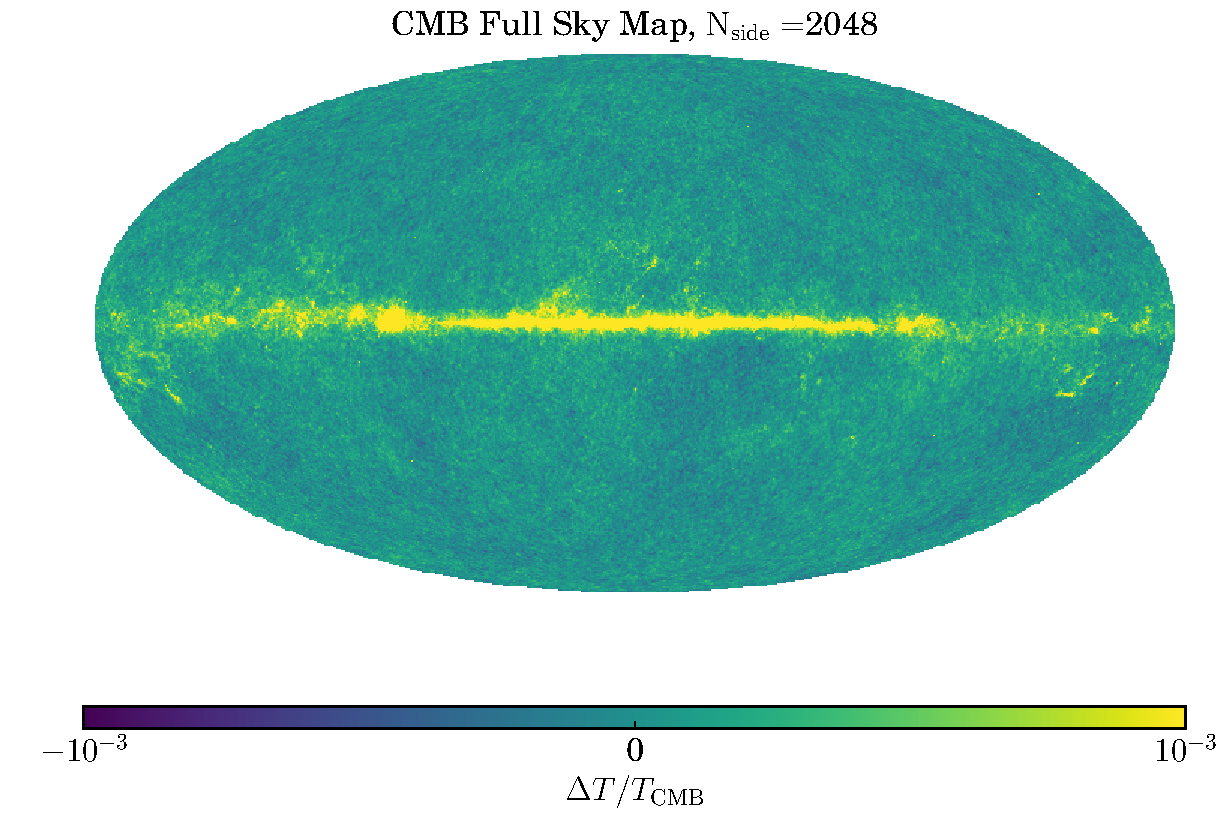
\includegraphics[width=0.49\linewidth]{figures/cmbfullsky.pdf} \hfill
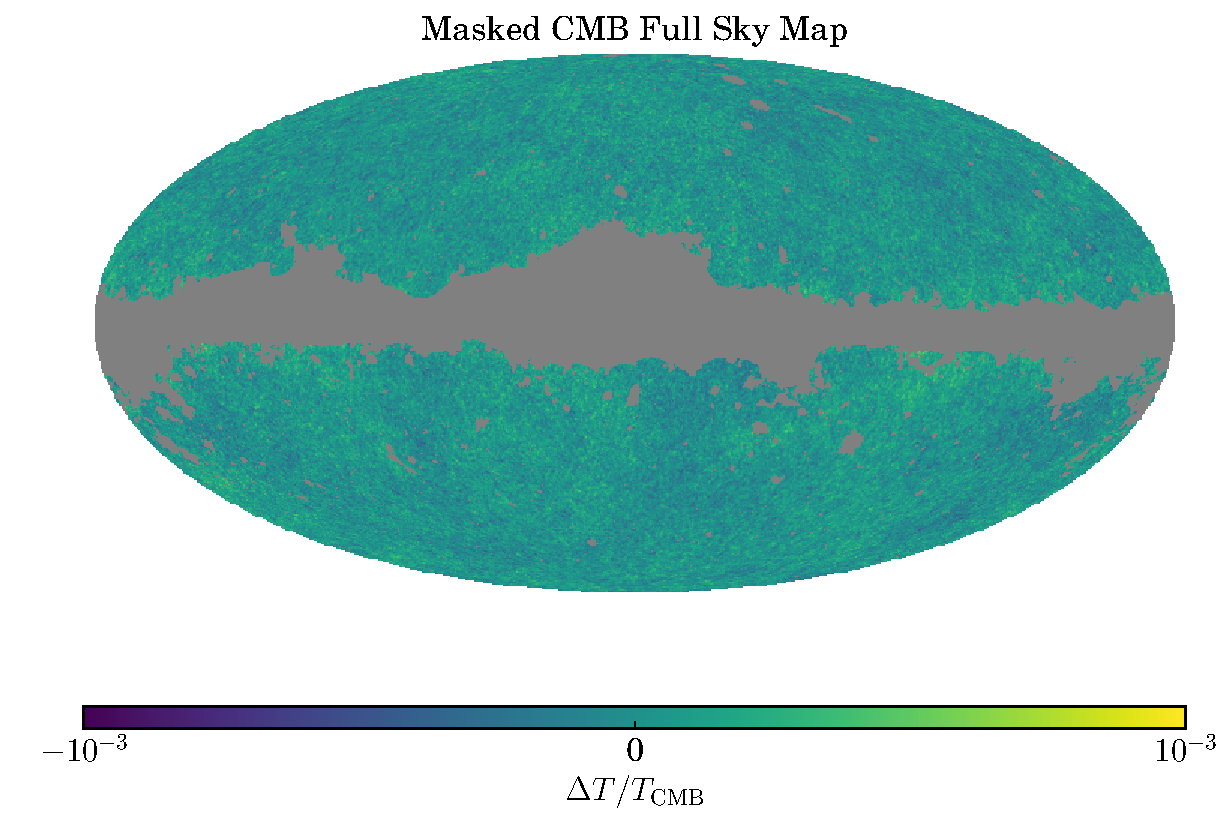
\includegraphics[width=0.49\linewidth]{figures/maskedfullsky.pdf}
\caption{The Planck PR3 100GHz Intensity Map of the CMB (Left) and the masked version, using the 2018 Intensity mask (Right).}\label{fig:cmbmaps}
\end{center}
\end{figure}


\section{Graph Networks}


The computations above, whilst providing perhaps an interesting representation of the data in their own right, were mainly done to provde input to a graph network. Learning based inference on such structured input has been recently pioneered as a means to push artificial intelligence forward \citep{DBLP:journals/corr/abs-1806-01261}. The collective reference for this is \textit{combinatorial generalisation}, where the system in question is biased towards certain, known, structural input. In our example, we make use of the natural correlation structure of the Ising model and the CMB pixel data.



\section*{Acknowledgements}



This work is based on observations obtained with Planck (\href{http://www.esa.int/Planck}{http://www.esa.int/Planck}), an ESA science mission with instruments and contributions directly funded by ESA Member States, NASA, and Canada.



\bibliography{main}
\end{document}
